\documentclass[12pt,a4paper]{book}
\usepackage[utf8]{inputenc}
\usepackage[portuguese]{babel}
\usepackage[T1]{fontenc}
\usepackage{amsmath}
\usepackage{amsfonts}
\usepackage{amssymb}
\usepackage{graphicx}
\usepackage{color}

\newtheorem{example}{Exemplo}

\usepackage[left=3cm,right=2cm,top=3cm,bottom=2cm]{geometry}
\title{Matemática Aplicada e Computacional}
\author{Eduardo José de Oliveira}

\newcommand{\todo}[1]{
	{\color{red}#1}
}

\begin{document}

\chapter{Introdução}

As fases na resolução de problemas em matemática aplicada e computacional que surgem nas mais diversas áreas do conhecimento, de modo geral, podem ser representadas da seguinte maneira:

\begin{figure}[h]
	\centering
	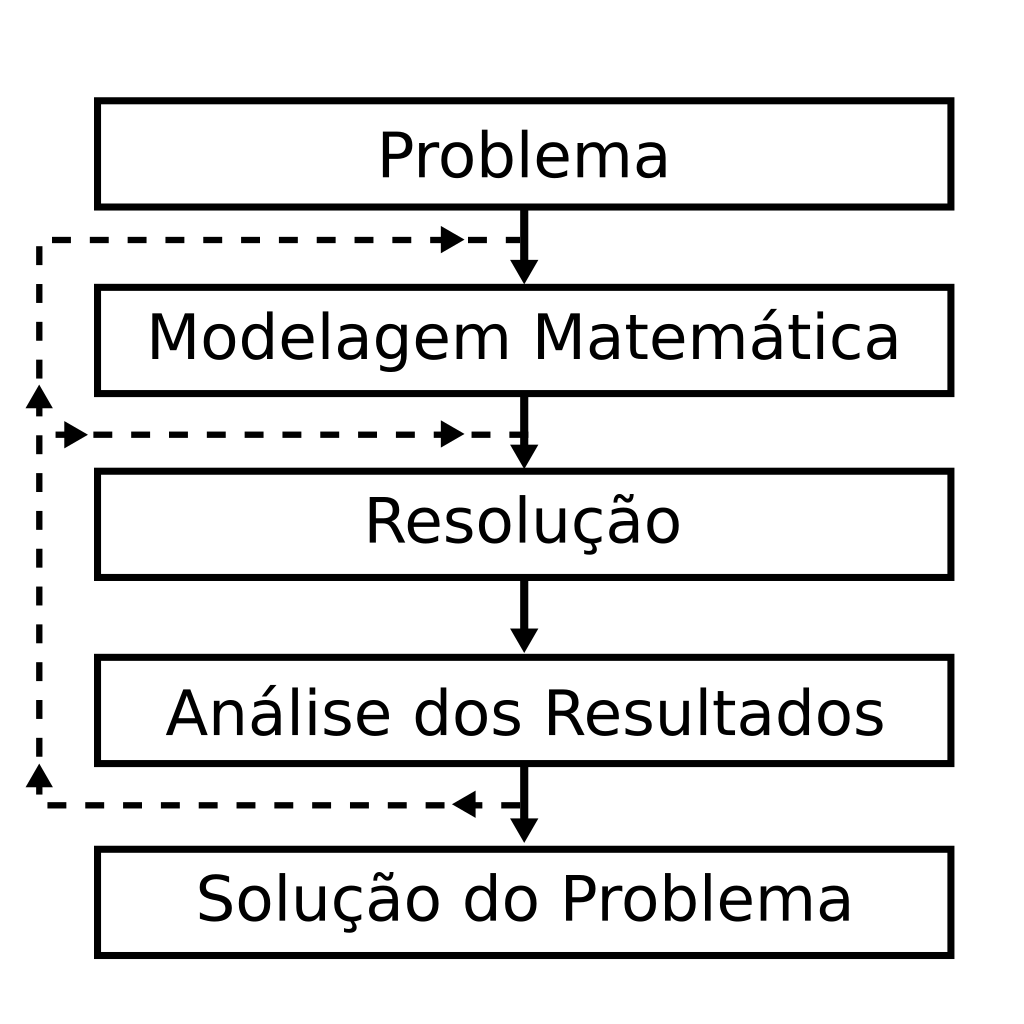
\includegraphics[scale=0.2]{figuras/figura_001}
	\caption{Fluxograma das fases na resolução de problemas em Matemática Aplicada e Computacional.}
\end{figure}

A primeira fase consiste basicamente em definir corretamente o problema a ser solucionado. A fase da modelagem matemática é onde ocorre a construção ou definição do modelo matemático que irá descrever o comportamento do problema em questão. Na fase de resolução são definidos e implementados os métodos para obtenção da solução do problema.

A análise dos resultados tem por finalidade verificar os resultados obtidos na resolução do problema. Se o resultado for satisfatório aceitamos a solução do problema, caso contrário, deve-se procurar outros métodos ou refazer a modelagem matemática.

\chapter{Principais erros na resolução de um problema}

Na resolução de um problema os erros podem surgir em cada fase. A seguir apresentamos os principais:

\begin{enumerate}
	\item \textbf{Erros na fase do problema:} Não definir corretamente o problema é um erro grave que pode levar a falsos resultados.
	
	\item \textbf{Erros na modelagem matemática:} O modelo matemático para um problema real deve representar o fenômeno que ocorre no mundo físico, porém, nem sempre é fácil. Normalmente são necessárias simplificações no modelo físico para se obter um modelo matemático (tratável) que fornecerá uma solução para o problema. Essas simplificações se constituem em fonte de erros, o que pode acarretar na necessidade de reformular o modelo matemático adotado.
\end{enumerate}

\begin{example}
	Um matemático quer determinar a altura de um edificio dispondo de uma esfera de metal, um cronômetro e a equação $s=s_0+v_0 t+ \frac{1}{2}at^2$. Para isso, ele sobe no topo do edificio e solta a esfera de metal anotando o tempo até a mesma tocar o solo, ou seja, 3 segundos.
	
	\begin{figure}[h]
		\centering
		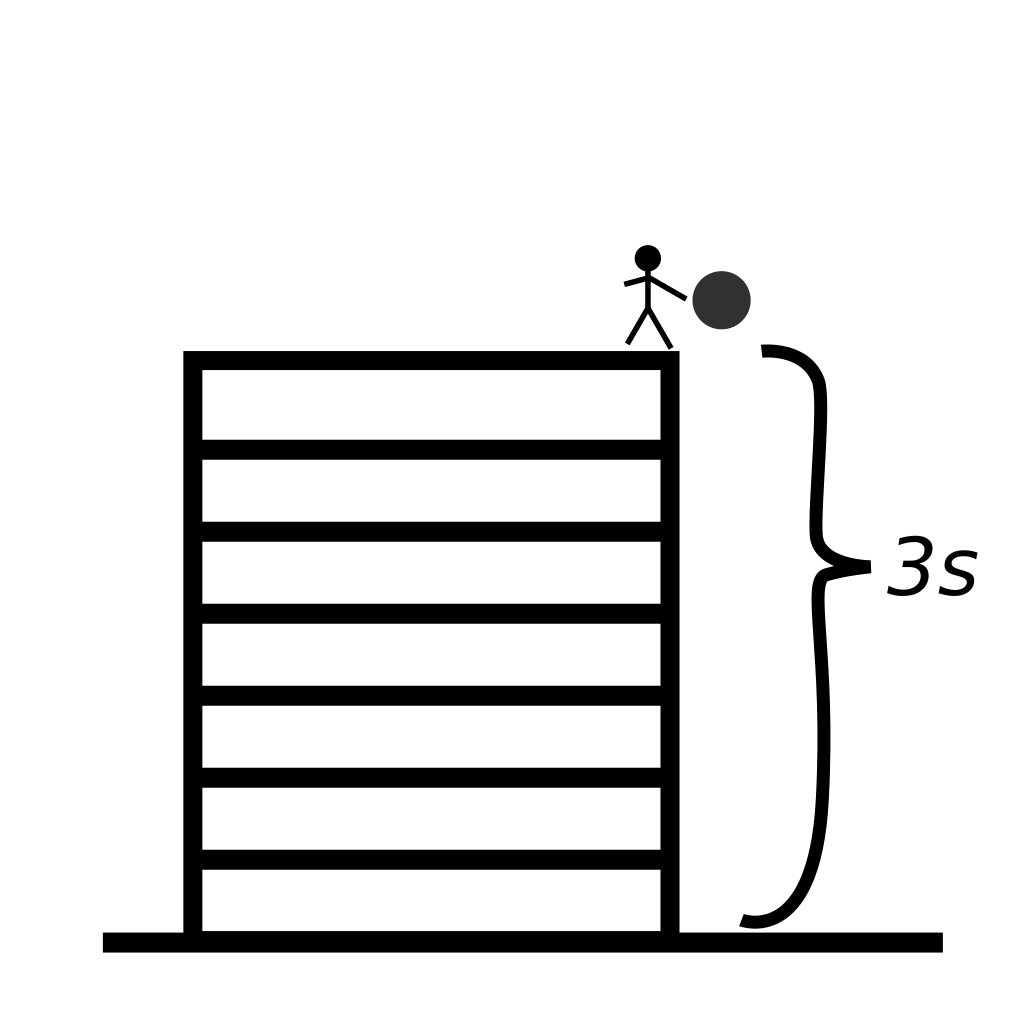
\includegraphics[scale=0.15]{figuras/figura_002}
	\end{figure}
	
	Logo, tem-se $s=s_0+v_0 t+\frac{1}{2}at^2=0+0\cdot 3 + \frac{1}{2}\cdot 9,8 \cdot 3^2=44,1$ m.
	
	Esse resultado é confiável?
	
	Provavelmente não, pois o modelo matemático utilizado não considera outras variáveis relevantes como, por exemplo, a resistência do ar, a velocidade do vento dentre outras.
	
	Além disso, há outro fato que pode influenciar diretamente a precisão na leitura do cronômetro, pois uma pequena variação nessa leitura pode acarretar uma grande variação no cálculo da altura do edificio. Se o tempo medido fosse de 3,5 segundos ao invés de 3 segundos, a altura do edificio seria calculada em 60,025 m. Ou seja, uma variação de 16,67\% na leitura do cronômetro ocasiona uma variação de 36,11\% no cálculo da altura do edifício.
	
	Logo pode-se notar a influência que o modelo matemático e a precisão dos dados de entrada exercem sobre a confiabilidade dos resultados.
\end{example}

\todo{Falar sobre a atividade na sala com a bolinha e a porta.}

\end{document}